%\chapter{Supercondensadores}
El almacenar energía eléctrica es uno de los mayores problemas a la hora de diseñar sistemas electrónicos tanto móviles como estacionarios, los requerimientos varían de acuerdo a las necesidades de cada uno, en general es un \textit{trade-off} entre densidad de energía (cuánta energía se puede almacenar) y densidad de potencia (que tan rápido puede ser entregada la energía almacenada). Las celdas de combustible (\textit{Fuel Cells}), entregan la mayor densidad de energía, pero son complicadas, mientras que las baterías poseen mayor densidad de potencia, pierden capacidad con los ciclos de carga y descarga. Los supercondensadores van un paso más allá, aumentado la densidad de potencia y aportando mayor vida útil, entregando una nueva posibilidad a la hora de diseñar sistemas eléctricos, ya como fuente de energía por sí mismo, o en sistemas híbridos combinados con otras tecnologías\citep{Thounthong2009}. Se utiliza el diagrama de Ragone (ver figura \ref{fig:ragone}), para comparar las diferentes tecnologías de almacenamiento de energía. 

\begin{figure}
	\centering
	\fbox{
		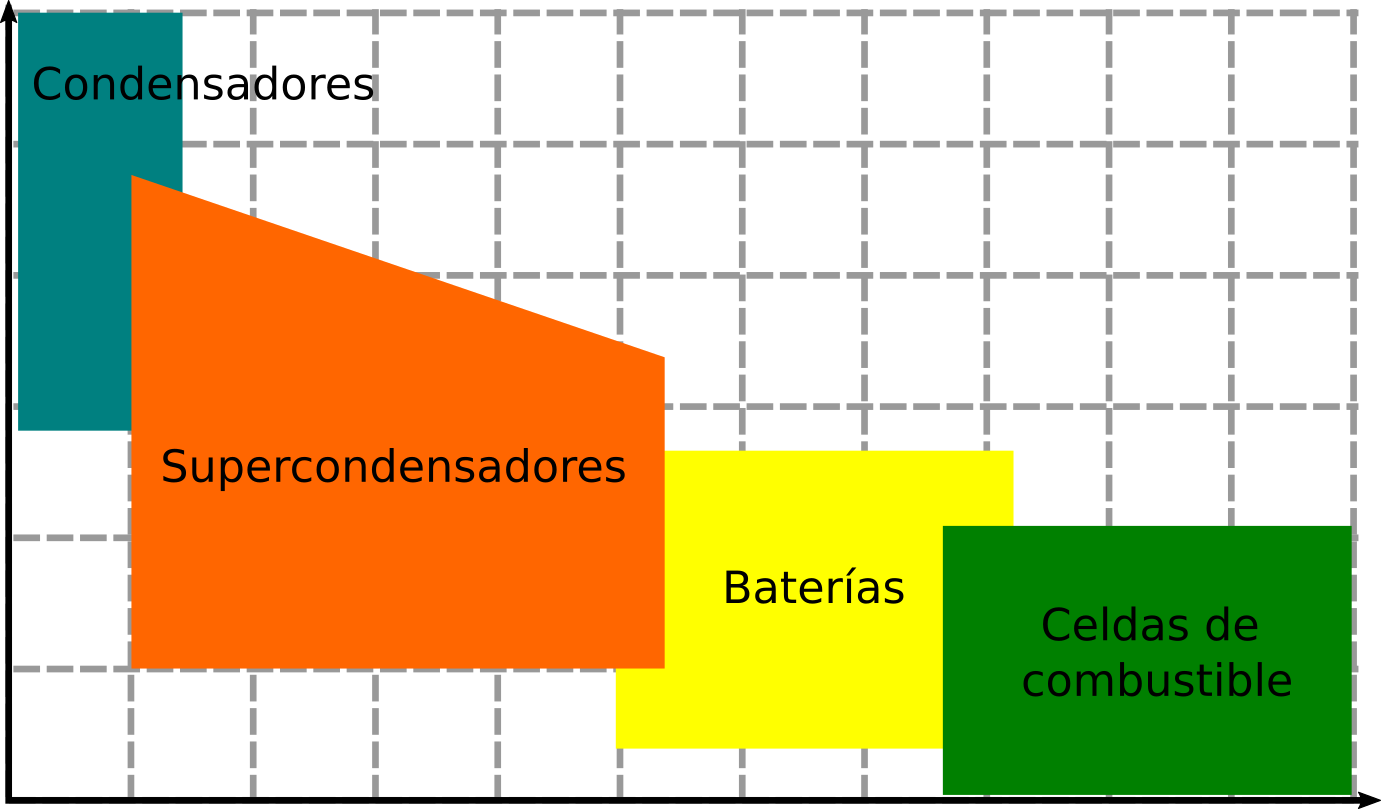
\includegraphics[width = 0.7\textwidth]{ragone.png}
	}
	\caption[Diagrama de Ragone]{El diagrama de Ragone compara diferentes tecnologías de almacenamiento de energía de acuerdo a su densidad de potencia y densidad de energía. }
	\label{fig:ragone}
\end{figure}

\section{El condensador ideal\index{condensador ideal}}
Generalmente un condensador se modela como un par de placas paralelas separadas por un dieléctrico, este es definido por su capacitancia, la que refleja la capacidad de almacenar energía. Del modelo de placas paralelas se desprende la definición de capacitancia $C$ como la razón entre la magnitud de carga en cada placa $Q$ y el voltaje entre los terminales $V$:

\begin{equation}
	C = \frac{Q}{V}
\end{equation}

Para fines prácticos, el condensador ideal como componente electrónico es modelado por la ecuación que relaciona la corriente\footnote{En estricto rigor, no hay corriente en el condensador, pues los electrones no ``saltan'' de una placa a otra, solo se acumulan en una de ellas. La corriente en el condensador, es más bien una corriente de desplazamiento.} con el voltaje en los terminales del dispositivo, considerando que $i = dq/dt$:

\begin{equation}
	i(t) = C \frac{dv(t)}{dt}
\end{equation}

Para corrientes constantes, el voltaje varía linealmente como en el gráfico de carga y descarga de la figura \ref{fig:plot:charge-discharge_ideal_cap}.
\begin{figure}[h!]
	\centering
	\fbox{
		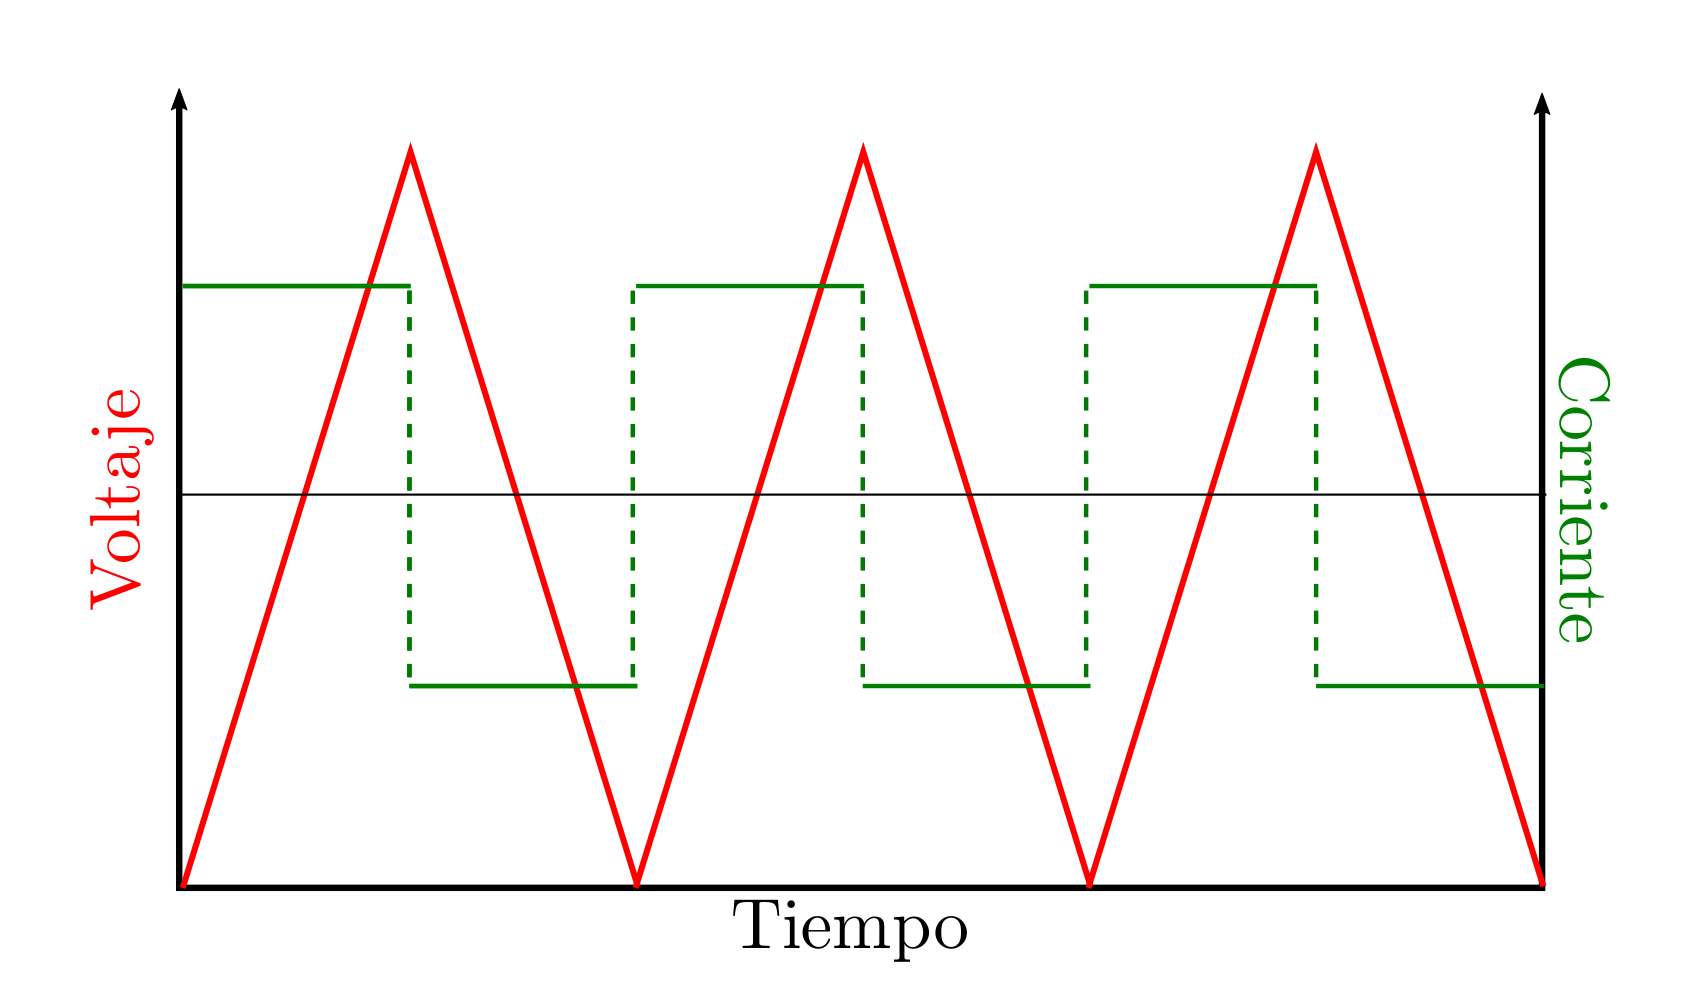
\includegraphics[width=0.7\textwidth]{charge-discharge_ideal_cap.png}
		}
	\caption{Carga y descarga de un condensador ideal a corriente constante.}
	\label{fig:plot:charge-discharge_ideal_cap}
\end{figure}

\section{El condensador real}
Un condensador ideal almacenaría energía al cargase y la entregaría al descargarse sin ninguna disipación, es decir, su eficiencia sería del 100\%, podría soportar cualquier voltaje aplicado o cargarse y descargarse por una corriente cuan grande se desee.  En realidad, los condensadores sí disipan energía, poseen voltajes de operación y corrientes máximas de carga y descarga. Todo esto depende de como fue construido y qué materiales se utilizaron.

\subsection{Breakdown voltage}
Los condensadores convencionales construidos con materiales dieléctricos están sujetos a un voltaje máximo de operación determinado por la tensión de ruptura (\textit{Breakdown voltage}), voltaje al cual se pierden las propiedades dieléctricas del material ocasionando cortocircuito al interior del dispositivo, está determinado por la fuerza dieléctrica del material y el espesor de este. En los condensadores electrolíticos la tensión de ruptura es determinada por otros mecanismos\citep{Yahalom1971}. En lo que respecta a los supercondensadores, el voltaje máximo de carga depende fundamentalmente de electrolíto usado, principalmente por las reacciones que ocurren a ciertos potenciales.\\


\subsection{Resistencia en serie equivalente (ESR)}
Las imperfecciones en la construcción de los electrodos, y la naturaleza de los materiales utilizados (e.g. resistencia no cero), disipan energía durante la carga y descarga como si se tratase de una resistencia en serie al condensador, esto se ve reflejado como una caída de voltaje en los terminales del dispositivo (figura \ref{fig:plot:charge-discharge_esr}), y disminuye la eficiencia de éste.

\begin{figure}[h!]
	\centering
	\fbox{
		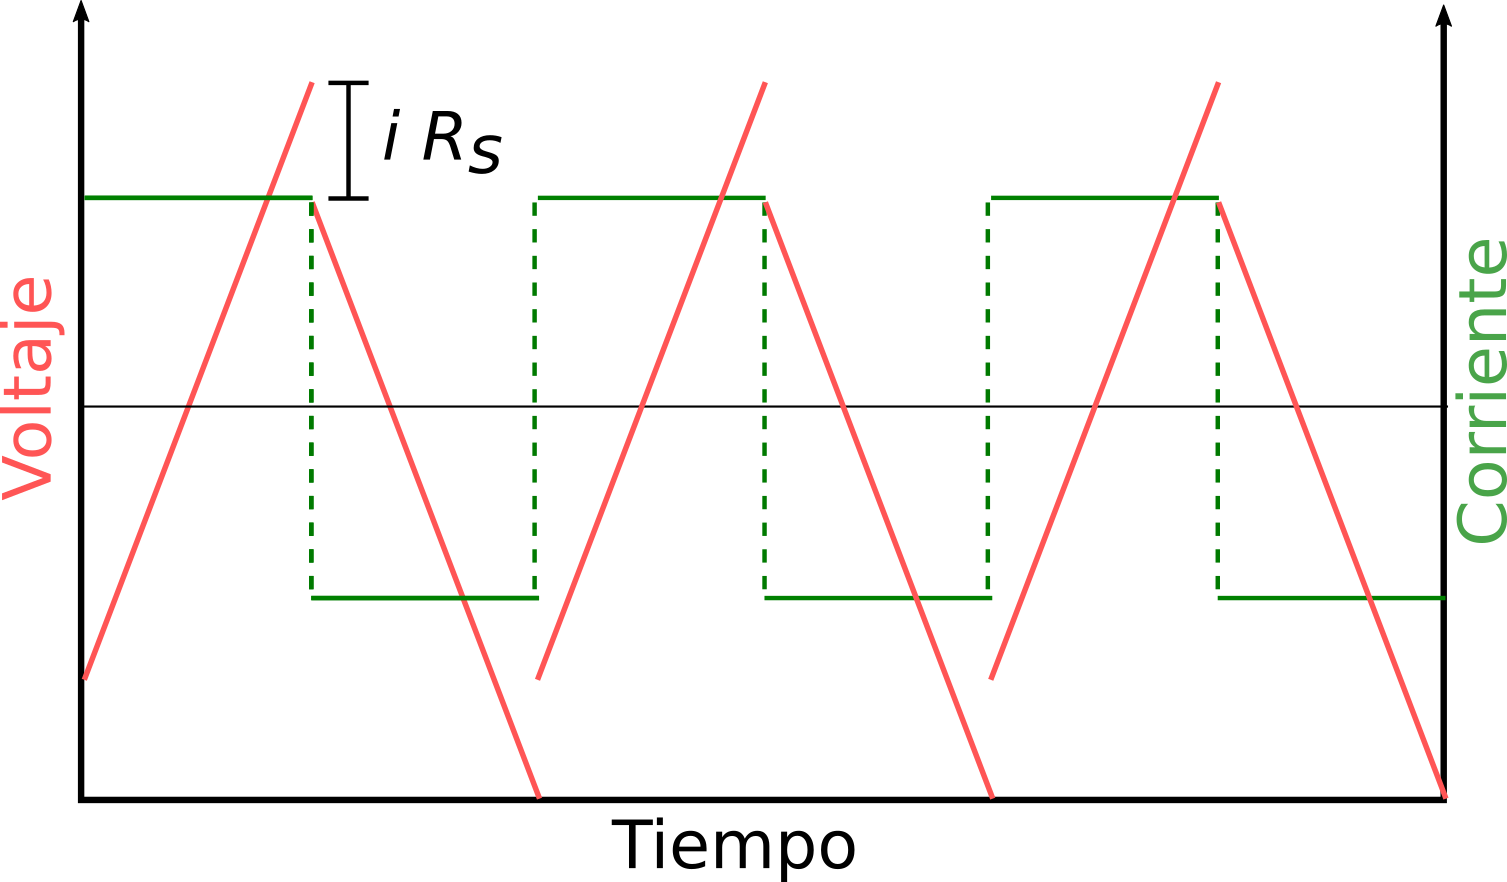
\includegraphics[width=0.7\textwidth]{charge-discharge_esr.png}
	}
	\caption{Carga y descarga de un condensador evidenciando el efecto de una ESR.}
	\label{fig:plot:charge-discharge_esr}
\end{figure}

\subsection{Corriente de fuga (\emph{leakage current})}
Entre los electrodos del condensador fluye una corriente no deseada cuando existe una diferencia de potencial entre los electrodos (cuando el condensador está cargado), esta corriente descarga al condensador incluso si está desconectado. Esta imperfección es modelada como una resistencia en paralelo al condensador.

\subsection{Circuito equivalente}
El comportamiento de los condensadores reales (convencionales o electroquímicos), son modeladas por un circuito equivalente, donde se introducen componentes que representan las imperfecciones del funcionamiento del condensador real.\\

\section{¿Qué hace a un supercondensador super?}
La densidad de energía de un supercondensador comparada a la de un condensador convencional es varios órdenes de magnitud superior, a modo de comparación, generalmente se utilizan microfaradios (10$^{-6}$ Faradios), para medir la capacidad de un condensador convencional, mientras que en un supercondensador es común ver capacidades de cientos de Faradios. Esta característica le otorga el grado de super a los supercondensadores.

\subsection{Doble capa electrostática de Helmholtz\index{doble capa de Helmholtz}}
La gran densidad de energía de un supercondensador tiene que surgir de algún mecanismo de almacenamiento de cargas. A diferencia de las baterías, este mecanismo es puramente físico, pues no hay reacciones químicas en los electrodos, las cargas son separadas en lo que Helmholtz llamó \emph{Doble capa electrónica} \citep{Frackowiak2001}, así, los supercondensadores también son llamados EDLCs (del inglés \emph{Electric Double Layer Capacitor}).

\begin{figure}[h!]
	\centering
	\fbox{
		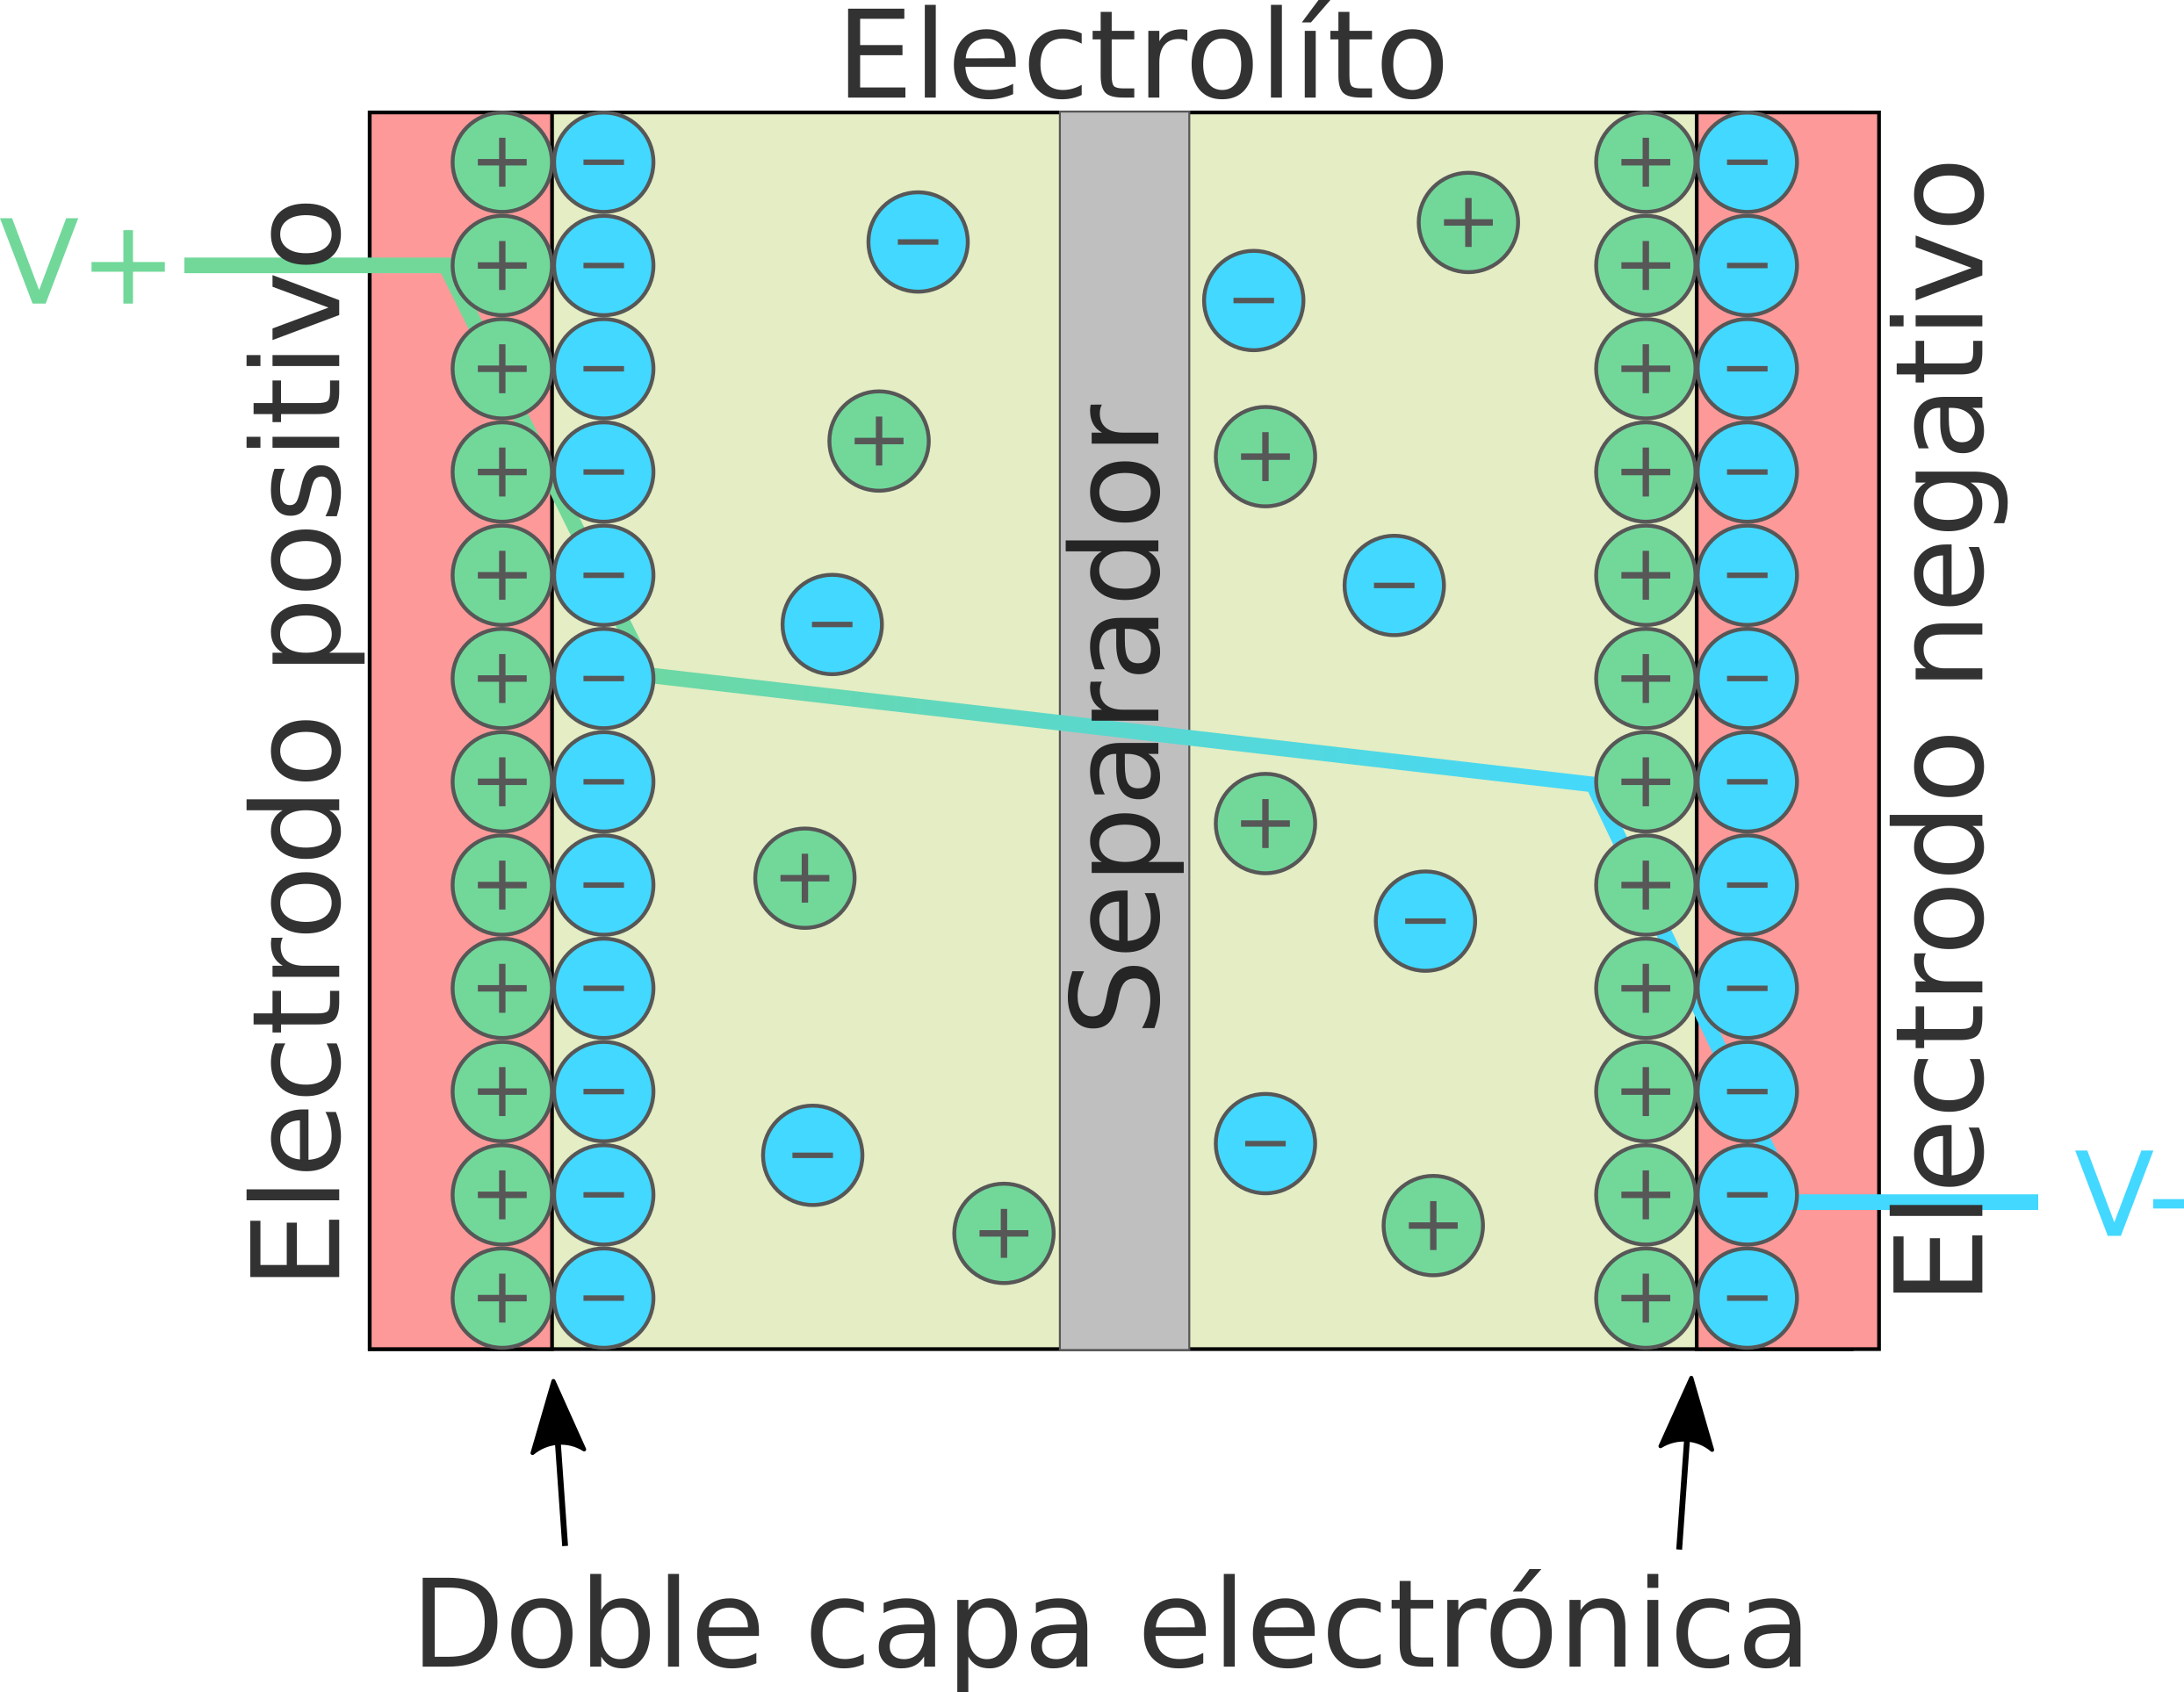
\includegraphics[width=0.7\textwidth]{edlc_schem.png}
		}
	\caption{Esquema de un supercondensador mostrando una doble capa electrónica de Helmholtz en cada electrodo.}
	\label{fig:edlc}
\end{figure}

\subsection{Pseudocapacitancia}
Cuando en un supercondensador existe intercambio de electrones entre los electrodos y el electrolítico (reacciones farádicas), se habla de pseudocapacitancia. El intercambio de electrones 


\section{Mediciones en supercondensadores}

\subsection{Voltametría cíclica}
En una voltametría cíclica convencional, se varía el potencia entre los electrodos de manera lineal y se registra la corriente, típicamente el barrido de voltaje se realiza entre dos voltajes fijos, y el recorrido se hace de ida y vuelta. Los parámetros importantes en la voltametría cíclica son: voltajes límite inferior y superior, velocidad de barrido.

\subsection{Espectroscopía de impedancia electroquímica}


\subsection{Carga y descarga cíclica}
Generalmente la carga y descarga ser realizan a corriente constante hasta alcanzar cierto voltaje umbral. La cantidad de ciclos puede llegar hasta 100.000 para estudiar la retención de la capacidad inicial del dispositivo.